\section*{4. Mini Lab - Similarity Meets Classification}

資料切分採用 0.25 的 test fraction、
random state 42 與 stratification；所有模型均為最大深度 3、random state 2 的
decision tree。

\begin{enumerate}
  \item Iris 資料集共有 150 筆資料與 4 個輸入特徵。類別名稱為 setosa、
  versicolor 與 virginica，各有 50 筆。切分所用的 random state 為 42，
  切分後有 112 筆訓練資料與 38 筆測試資料。

  \item StandardScaler 僅使用 112 筆訓練資料進行擬合，再分別轉換訓練集與測試集。
  兩個模型的比較如下。

  \begin{center}
  \small
  \rowcolors{2}{lightrow}{white}
  \begin{tabular}{lllll}
    \toprule
    模型 & 根節點分割 & 葉節點 & 訓練準確率 & 測試準確率 \\
    \midrule
    原始資料 & petal width $\leq 0.8000$ cm & 5 & 0.9821 & 0.9211 \\
    標準化資料 & standardized petal width $\leq -0.5135$ & 5 & 0.9821 & 0.9211 \\
    \bottomrule
  \end{tabular}
  \end{center}

  兩棵樹的深度皆為 3，分支結構也相同。原始單位下，規則分別在 petal width
  的 0.80 與 1.70 cm，以及 petal length 的 4.95 與 4.85 cm 進行分割；
  標準化後相對應的門檻變為 $-0.51$、0.66、0.67 與 0.61。兩個模型對 38 筆
  測試資料的預測完全相同。

  標準化只改變門檻的數值座標，不會改變單一特徵內各觀測值的排序。Decision tree
  每次只在一個特徵上尋找切點，因此候選分割仍然相同。Euclidean distance 則會把
  不同特徵的座標差合併計算；改變任一特徵的尺度，就會改變該特徵對總距離的貢獻，
  進而可能改變 nearest neighbors。

  \item 原始 decision tree 的 training accuracy 為 0.9821，test accuracy
  為 0.9211。這個差距表示模型在未見資料上的表現略有下降。若 training accuracy
  遠高於 test accuracy，通常代表 overfitting：模型學到了訓練資料中的偶然邊界或
  雜訊，卻無法推廣至新資料。可透過限制深度、pruning，或利用驗證資料選擇
  hyperparameters 來改善。

  \item 由原始訓練集以 random state 42 抽取 stratified subsets，並保持測試集不變。

  \begin{center}
  \small
  \rowcolors{2}{lightrow}{white}
  \begin{tabular}{rrrrrr}
    \toprule
    比例 & 訓練筆數 & 根節點特徵 & 門檻 & 深度 / 葉節點 & 測試準確率 \\
    \midrule
    20\%  & 22  & Petal width & 0.80 & 3 / 4 & 0.9211 \\
    40\%  & 44  & Petal width & 0.70 & 3 / 4 & 0.9211 \\
    60\%  & 67  & Petal width & 0.70 & 3 / 4 & 0.9737 \\
    80\%  & 89  & Petal width & 0.80 & 3 / 5 & 0.9211 \\
    100\% & 112 & Petal width & 0.80 & 3 / 5 & 0.9211 \\
    \bottomrule
  \end{tabular}
  \end{center}

  所有訓練資料量下，第一個分割特徵皆為 petal width，但門檻會在 0.70 與
  0.80 cm 之間變動。樹深固定為允許的最大值 3，葉節點數則在 80\% 時由 4 增為 5。
  測試準確率大多維持 0.9211，只有 60\% 的子集達到 0.9737。因此，增加訓練資料
  並不保證決策樹會更深或準確率會單調提高。不同樣本可能改變 impurity-optimal
  threshold 與下層分支，而固定的 depth limit 也限制了模型複雜度。

  \begin{figure}[ht]
    \centering
    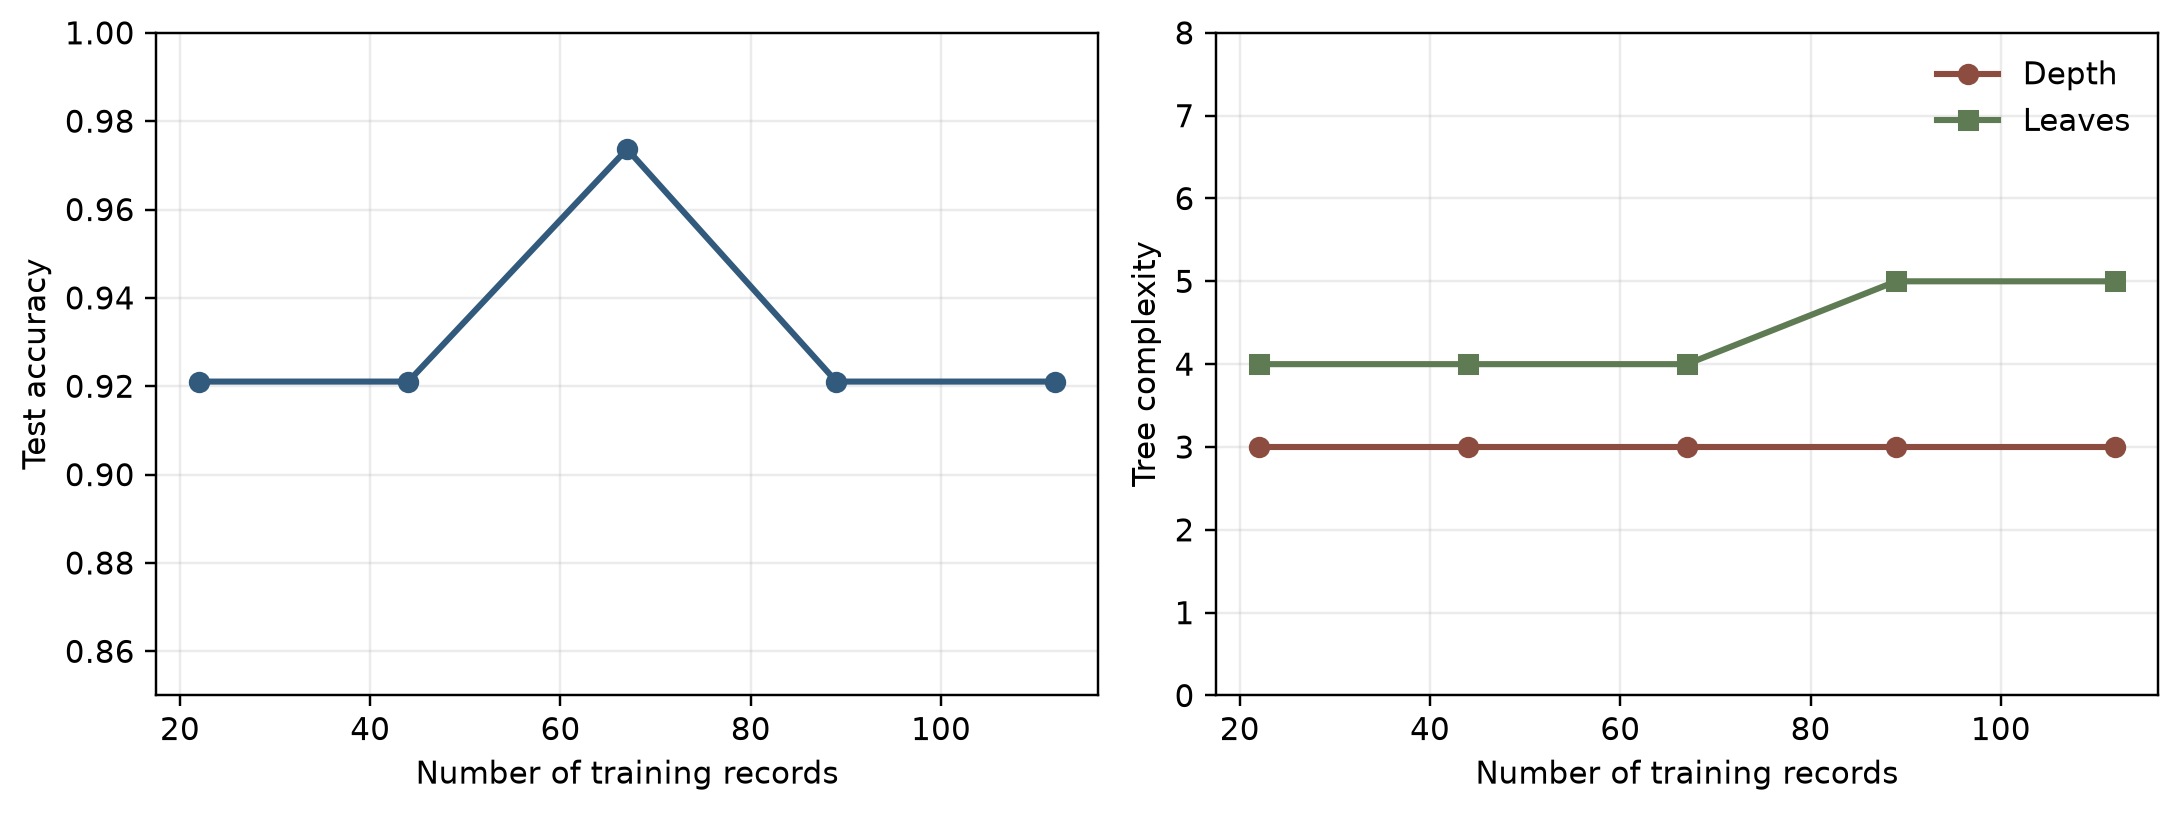
\includegraphics[width=0.94\linewidth]{q4_training_size.png}
    \caption{固定測試集下，訓練資料量、測試準確率與決策樹複雜度的關係。}
  \end{figure}

  \item \textbf{綜合說明（內容對應英文版 131 words）。}
  標準化改變了分割門檻的數值，卻沒有改變 decision tree 所選的特徵、資料分區、
  預測結果或準確率。這與 axis-aligned tree 的運作方式一致：單調的尺度轉換會保留
  特徵內部的數值順序。Euclidean-distance neighbors 的情況不同，因為特徵尺度會
  直接改變合併後的距離。原始模型的訓練準確率為 0.982、測試準確率為 0.921，
  兩者只有小幅 generalization gap；若差距很大，才較可能表示 overfitting。
  在不同大小的 stratified training subsets 中，petal width 始終是根節點特徵，
  但門檻與葉節點數會改變。測試準確率在 60\% 訓練資料時最高，之後又回到原來水準。
  因此，更多資料不一定單調增加樹深或準確率；sampling variation 會改變最佳分割，
  固定的 depth limit 則會限制模型複雜度。
\end{enumerate}
